\documentclass[11pt,a4paper]{article}

\usepackage[T1]{fontenc}
\usepackage{lmodern}
\usepackage[margin=2.3cm]{geometry}
\usepackage{amsmath,amssymb}
\usepackage{graphicx}
\usepackage{booktabs}
\usepackage{multirow}
\usepackage{xcolor}
\usepackage[font=small,labelfont=bf]{caption}
\usepackage{tikz}
\usetikzlibrary{positioning,arrows.meta,fit,backgrounds,calc}
\usepackage[numbers,sort&compress]{natbib}
\usepackage[hidelinks]{hyperref}
\usepackage{microtype}
\usepackage[section]{placeins}

\definecolor{ink}{HTML}{14213D}
\definecolor{blue}{HTML}{2B6CB0}
\definecolor{lblue}{HTML}{DCEBFA}
\definecolor{grey}{HTML}{EEF2F8}
\definecolor{orange}{HTML}{C05621}
\definecolor{lorange}{HTML}{FCEBDD}

\newcommand{\cube}[1]{#1^3}
\newcommand{\x}{\ensuremath{\times}}

\title{\textbf{Validating for the Unseen: Self-Supervised 3D Light-Sheet Microscopy Segmentation with Unseen-Type Model Selection and Foreground Calibration}\\[4pt]
\large Solution of team \emph{Four and Furious} for the SELMA3D 2026 challenge}

% TODO: complete the author list, affiliations and corresponding e-mail before submission.
\author{Ayush Gupta\textsuperscript{1} \and [Co-author]\textsuperscript{1} \and [Co-author]\textsuperscript{1}\\[4pt]
\small \textsuperscript{1}[Affiliation, city, country] \quad Corresponding author: [e-mail]}

\date{}

\begin{document}
\maketitle

\begin{abstract}
Segmenting cells, plaques, nuclei, vessels and nerves in cleared-tissue light-sheet microscopy (LSM) requires models that transfer to structure types for which no annotation exists. The SELMA3D 2026 challenge formalises this setting: networks are pretrained without labels on 3,400 unannotated volumes of 17 structure types and fine-tuned on only 82 annotated patches, while most test volumes show structure types absent from the annotations. We describe our solution and, more importantly, what we learned about validating models for unseen structure types. Our network is a residual 3D U-Net ensemble initialised by \emph{signal-weighted masked reconstruction}, a masked-image pretext task in which structure voxels dominate the loss, and fine-tuned with a recipe selected on a \emph{leave-family-out} proxy that withholds two structure families. We report three findings. (i) A held-out split of annotated volumes failed to predict the preliminary-test score---it favoured the weaker of our two best models---whereas a label-free statistic---the amount of foreground a model predicts on unlabelled test volumes of unseen types, relative to a reference---tracked it. (ii) On withheld families, performance peaks early in training while seen-type accuracy keeps rising; re-thresholding shows this decline is \emph{miscalibration, not forgetting}: with the true amount of foreground, the fully trained model is better (0.432 vs.\ 0.413), but its foreground drifts in opposite directions for tubes (\x3.0) and cells (\x0.6). (iii) Test-time self-training reverses sign with object topology, helping every unseen tubular volume and hurting almost every unseen cell volume. On the final test set the method reached Dice 0.653 and clDice 0.738 on contiguous structures, with a standard deviation across volumes of about 0.15, and Dice 0.547 and PQ 0.360 on isolated structures.
\end{abstract}

% ------------------------------------------------------------------------------------------
\section{Introduction}

Tissue clearing combined with light-sheet fluorescence microscopy images whole organs at cellular resolution in three dimensions \cite{erturk2012disco,ueda2020clearing}. Quantifying what these volumes contain---activated neurons, amyloid plaques, nuclei, blood vessels, nerves---relies on 3D segmentation \cite{renier2016clearmap,todorov2020vessap}, and the number of stains, organs and species makes it impractical to annotate every structure type. Self-supervised learning (SSL) on unannotated volumes followed by fine-tuning on a few annotated ones is therefore an attractive recipe \cite{zhou2021modelsgenesis,tang2022swinunetr,he2022mae}. The SELMA3D challenge series evaluates exactly this recipe for LSM \cite{chen2025selma3d}. Its 2026 edition \cite{selma3d2026design} provides 3,400 unannotated volumes of 17 structure types for pretraining and 82 annotated patches of six types for fine-tuning; the preliminary test set contains 26 volumes of which 17 show structure types that have no annotated example (microglia, organ proteins, gut nerves, lymphatic vessels, axonal markers).

This paper describes our solution and the validation practice we arrived at. The central difficulty was not model capacity but \emph{model selection}: the usual practice of holding out annotated volumes measures accuracy on structure types the model has already seen, and in our hands it was not predictive of the preliminary-test score. Our contributions are:
\begin{itemize}
  \item A compact pipeline---signal-weighted masked-reconstruction pretraining, a fine-tuning recipe selected on unseen families, and a two-model 3D U-Net ensemble---trained on a single 8\,GB laptop GPU, reaching Dice 0.653 and clDice 0.738 on the contiguous structures of the final test set.
  \item Evidence that a \emph{label-free} unseen-type foreground statistic tracks preliminary-test performance where held-out accuracy does not, and a controlled experiment showing that late-training losses on unseen families are a calibration drift in opposite directions for tubes and cells, not a loss of discriminative ability.
  \item A morphology-aware router with per-volume \emph{foreground anchoring}, which lets larger-context experts refine contiguous structures without changing the amount of foreground, and an analysis of structure-conditional test-time self-training.
  \item A set of negative results (post-processing, test-time augmentation, ensembling and routing variants) that did not transfer to unseen types.
\end{itemize}

% ------------------------------------------------------------------------------------------
\section{Related work}

\paragraph{Self-supervised pretraining for 3D segmentation.} Restoration-based pretext tasks \cite{zhou2021modelsgenesis}, masked image modelling \cite{he2022mae,xie2022simmim} and multi-task pretraining of 3D transformers \cite{tang2022swinunetr} have all been used to initialise medical segmentation networks. Most were designed for CT or MRI, where the object of interest occupies a large fraction of the field of view. In cleared-tissue LSM the signal is sparse; we adapt masked reconstruction so that structure voxels dominate the objective.

\paragraph{Segmentation networks and metrics.} U-Net variants remain the reference architecture for volumetric segmentation \cite{ronneberger2015unet,cicek2016unet3d,isensee2021nnunet}; we use the residual DynUNet implementation of MONAI \cite{cardoso2022monai}. SELMA3D scores isolated structures with Dice and panoptic quality \cite{kirillov2019panoptic} and contiguous structures with Dice and centreline Dice \cite{shit2021cldice}, following recommendations to match metrics to object topology \cite{maierhein2024metrics}.

\paragraph{Model selection under distribution shift and calibration.} Domain-generalisation benchmarks show that model selection without access to the target distribution is a major source of error \cite{gulrajani2021domainbed}; leave-one-domain-out validation is the common remedy. Modern networks are often miscalibrated \cite{guo2017calibration}; we show that in segmentation of unseen structure types the relevant miscalibration is in the \emph{amount} of predicted foreground and that it can be corrected per volume without labels.

\paragraph{Test-time adaptation.} Test-time training \cite{sun2020ttt}, entropy minimisation \cite{wang2021tent} and pseudo-labelling \cite{lee2013pseudolabel} adapt a model to each test distribution. TopoTTA \cite{zhou2025topotta} specialises test-time adaptation to tubular structures. We report that plain confident-voxel self-training helps tubular and hurts blob-like unseen structures within one task.

% ------------------------------------------------------------------------------------------
\section{Challenge, data and metrics}

\begin{table}[!htbp]
\centering\small
\caption{Data used. All four collections are distributed by the challenge organisers through the BioImage Archive under CC~BY~4.0 \cite{data2110,data2106,data3281,data3277}. Fine-tuning used only the annotated patches, for both tasks.}
\label{tab:data}
\resizebox{\linewidth}{!}{%
\begin{tabular}{llrl}
\toprule
Set & Category & Volumes & Structure types (volume size in voxels) \\
\midrule
\multirow{2}{*}{Annotated (fine-tuning)} & isolated & 38 & amyloid plaques 20 ($300^3$), cell nuclei 9 ($200^3$), c-Fos neurons 9 ($200^3$) \\
 & contiguous & 44 & blood vessels 16 ($50\x500\x500$), peripheral nerves 16 ($400^3$), axons 12 ($250\x250\x100$--$120$) \\
\midrule
Unannotated (pretraining) & both & 3,400 & 17 types $\times$ 200 patches of $300^3$ (107.6\,GB), Fig.~\ref{fig:pool} \\
\midrule
\multirow{2}{*}{Preliminary test} & isolated & 12 & plaques 3, nuclei 1, c-Fos 1, \emph{microglia 3, organ proteins 4} \\
 & contiguous & 14 & vessels 2, peripheral nerves 2, \emph{gut nerve 4, lymphatic vessels 4, axonal markers 2} \\
\bottomrule
\end{tabular}}
\end{table}

\begin{figure}[!htbp]
\centering
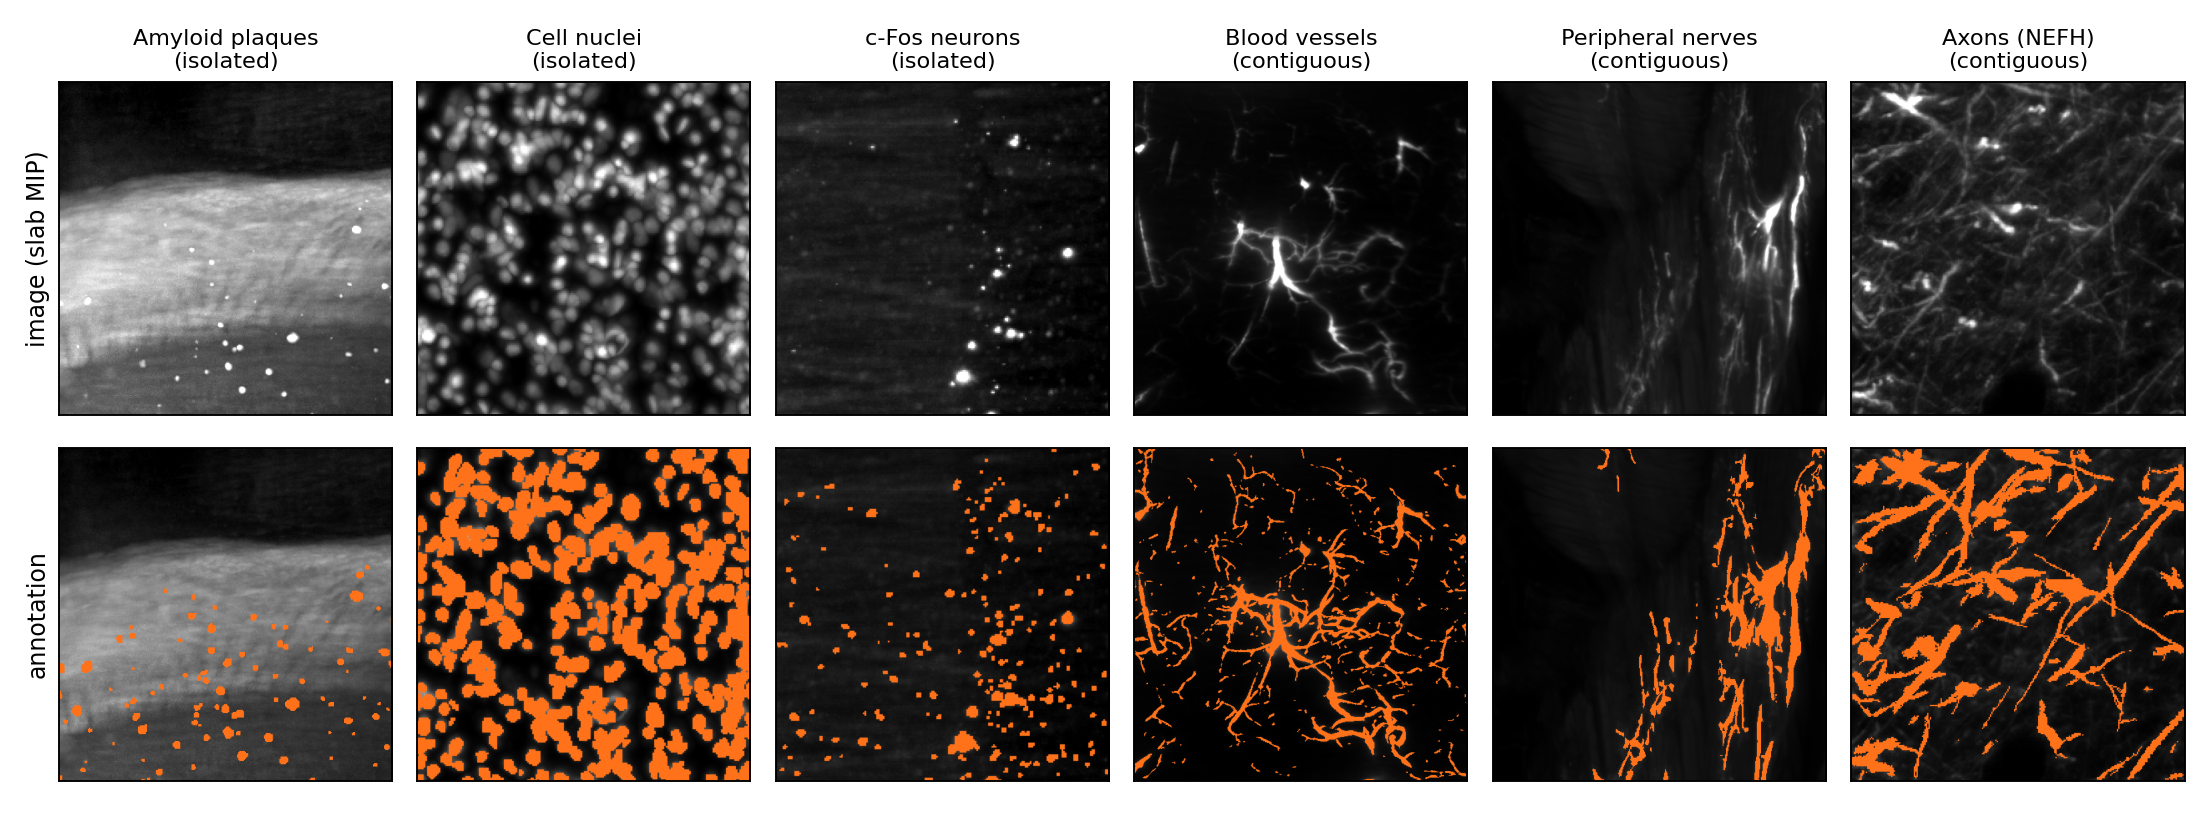
\includegraphics[width=\linewidth]{fig/dataset_annotated.png}
\caption{The six annotated structure types (top: slab maximum-intensity projection; bottom: annotation). Isolated structures are scored by object (panoptic quality), contiguous ones by topology (centreline Dice).}
\label{fig:annotated}
\end{figure}

\begin{figure}[!htbp]
\centering
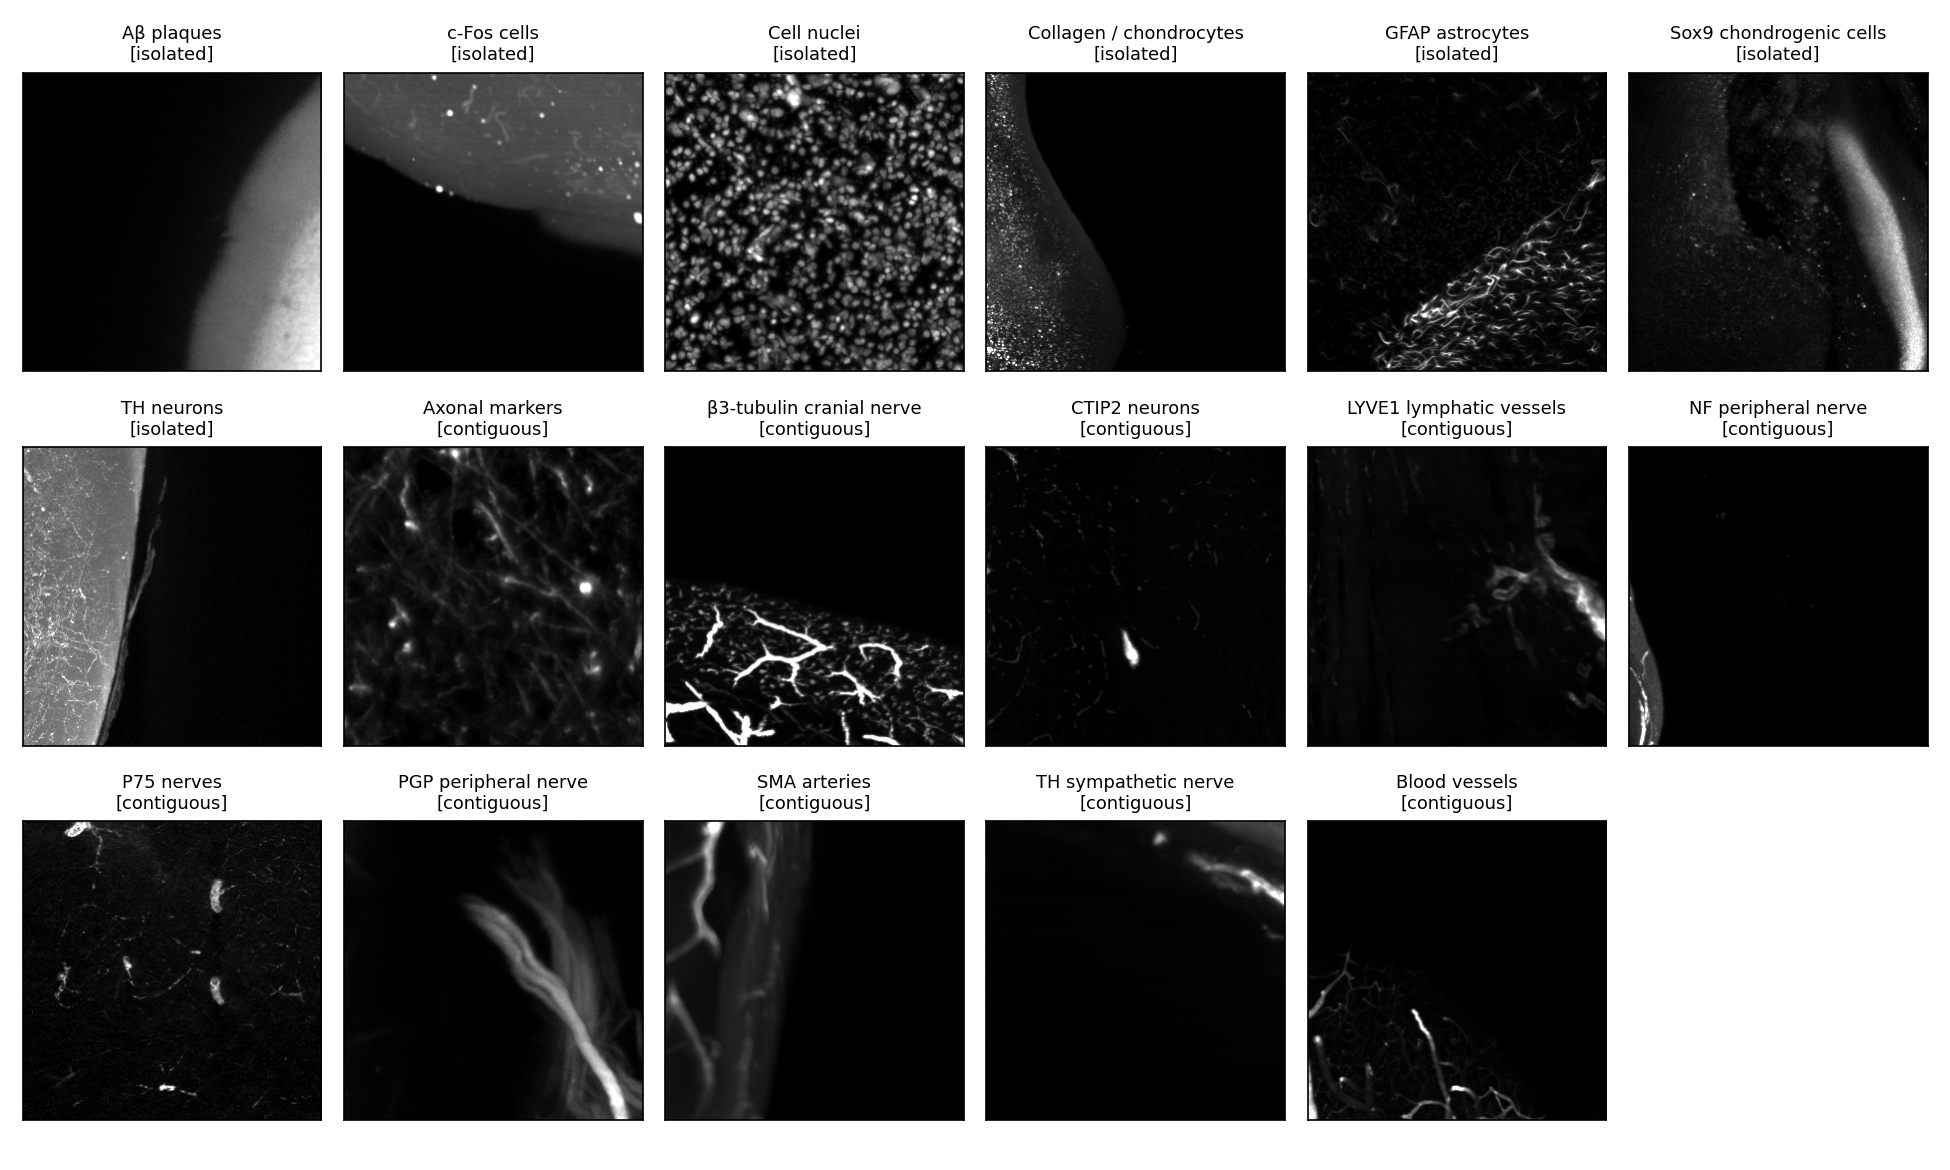
\includegraphics[width=\linewidth]{fig/dataset_pool.png}
\caption{One unannotated patch of each of the 17 structure types in the pretraining pool (slab maximum-intensity projection of the most structured of eight patches per type). Many types---astrocytes, chondrocytes, arteries, sympathetic and cranial nerves---have no annotated counterpart.}
\label{fig:pool}
\end{figure}

\paragraph{Tasks.} Task~1 fixes the pretraining data to the provided pool; Task~2 allows any additional unannotated data \cite{selma3d2026design}. In both tasks fine-tuning may use only the 82 annotated patches. We used the provided pool in both tasks and submitted to Task~1 and Task~2 the two variants described in Section~\ref{sec:method}. Table~\ref{tab:data} and Figs.~\ref{fig:annotated}--\ref{fig:pool} summarise the data.

\paragraph{Metrics.} For isolated structures, Dice (DSC) and panoptic quality (PQ, matching objects at IoU\,$>$\,0.5) \cite{kirillov2019panoptic}; for contiguous structures, Dice and centreline Dice (clDice) \cite{shit2021cldice}. Each metric is averaged over test volumes. Where we summarise with one number we use the mean of the four metrics.

\paragraph{Evaluation budget.} Each preliminary-test submission reveals four averaged numbers, and the number of submissions is small. Every design decision therefore had to be made on local validation, which is the subject of Section~\ref{sec:validation}.

% ------------------------------------------------------------------------------------------
\section{Method}
\label{sec:method}

\begin{figure}[!htbp]
\centering
\resizebox{\linewidth}{!}{%
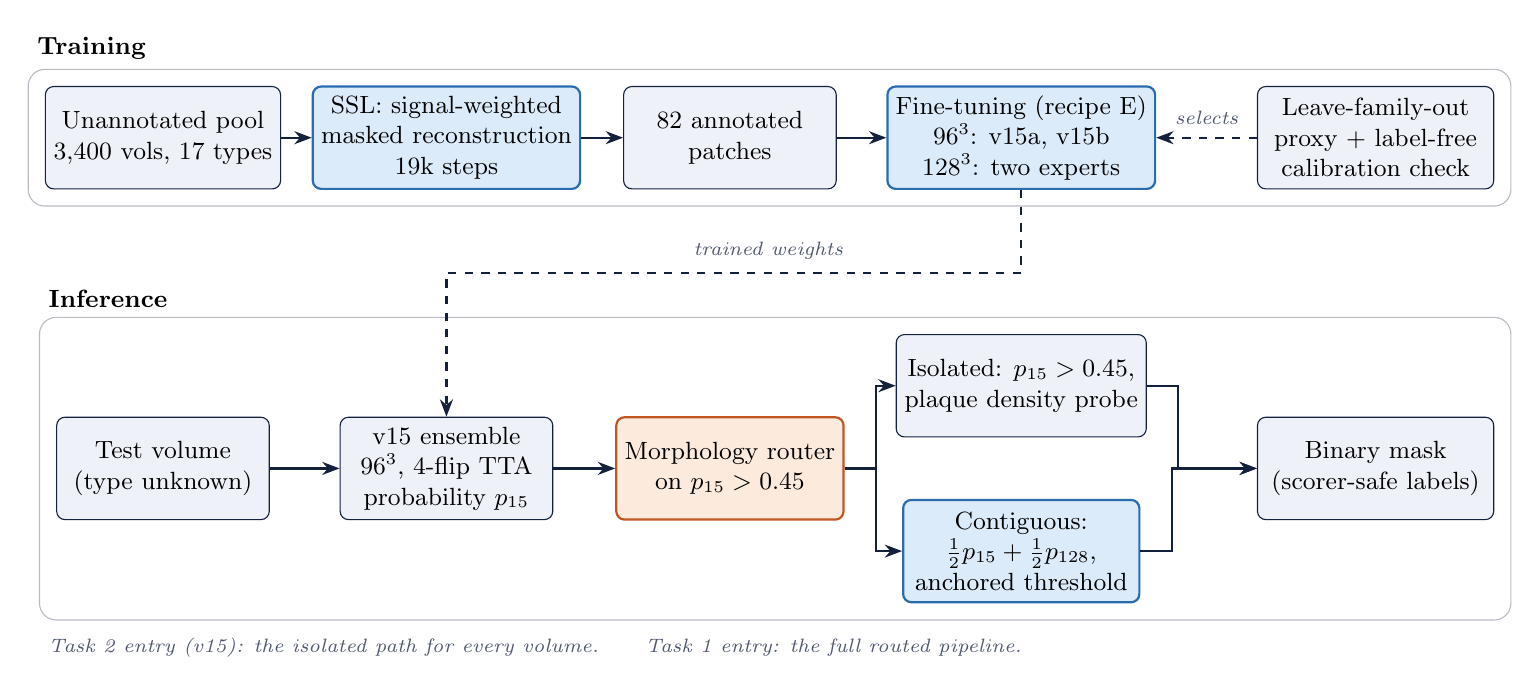
\begin{tikzpicture}[
  box/.style={draw=ink, rounded corners=3pt, align=center, font=\small, minimum height=13mm, minimum width=27mm, inner sep=3pt, fill=grey},
  new/.style={box, fill=lblue, draw=blue, line width=0.8pt},
  hot/.style={box, fill=lorange, draw=orange, line width=0.8pt},
  arr/.style={-{Stealth[length=2.2mm]}, line width=0.8pt, draw=ink},
  lab/.style={font=\scriptsize\itshape, text=ink!75}]
% ---------------- training
\node[box] (pool) at (0,0) {Unannotated pool\\3,400 vols, 17 types};
\node[new] (ssl) at (3.6,0) {SSL: signal-weighted\\masked reconstruction\\19k steps};
\node[box] (ann) at (7.2,0) {82 annotated\\patches};
\node[new, minimum width=30mm] (ft) at (10.9,0) {Fine-tuning (recipe E)\\$96^3$: v15a, v15b\\$128^3$: two experts};
\node[box, minimum width=30mm] (sel) at (15.4,0) {Leave-family-out\\proxy + label-free\\calibration check};
\draw[arr] (pool) -- (ssl);
\draw[arr] (ssl) -- (ann);
\draw[arr] (ann) -- (ft);
\draw[arr, dashed] (sel) -- node[lab, above=1pt]{selects} (ft);
% ---------------- inference
\node[box] (vol) at (0,-4.2) {Test volume\\(type unknown)};
\node[box] (v15) at (3.6,-4.2) {v15 ensemble\\$96^3$, 4-flip TTA\\probability $p_{15}$};
\node[hot] (router) at (7.2,-4.2) {Morphology router\\on $p_{15}>0.45$};
\node[box, minimum width=30mm] (iso) at (10.9,-3.15) {Isolated: $p_{15}>0.45$,\\plaque density probe};
\node[new, minimum width=30mm] (cont) at (10.9,-5.25) {Contiguous:\\$\tfrac12 p_{15}+\tfrac12 p_{128}$,\\anchored threshold};
\node[box, minimum width=30mm] (mask) at (15.4,-4.2) {Binary mask\\(scorer-safe labels)};
\draw[arr] (vol) -- (v15);
\draw[arr] (v15) -- (router);
\draw[arr] (router.east) -- ++(4mm,0) |- (iso.west);
\draw[arr] (router.east) -- ++(4mm,0) |- (cont.west);
\draw[arr] (iso.east) -- ++(4mm,0) |- (mask.west);
\draw[arr] (cont.east) -- ++(4mm,0) |- (mask.west);
\draw[arr, dashed] (ft.south) -- ++(0,-1.05) -| node[lab, pos=0.22, above=1pt]{trained weights} (v15.north);
\begin{scope}[on background layer]
\node[fit=(pool)(sel), draw=ink!30, rounded corners=6pt, inner sep=6pt] (tr) {};
\node[anchor=south west, font=\small\bfseries] at (tr.north west) {Training};
\node[fit=(vol)(mask)(iso)(cont), draw=ink!30, rounded corners=6pt, inner sep=6pt] (inf) {};
\node[anchor=south west, font=\small\bfseries] at (inf.north west) {Inference};
\end{scope}
\node[lab, anchor=north west] at ($(inf.south west)+(0,-1mm)$) {Task 2 entry (v15): the isolated path for every volume.\qquad Task 1 entry: the full routed pipeline.};
\end{tikzpicture}}
\caption{Overview. Blue: components introduced in this work; orange: the morphology router. The Task~2 entry (v15) segments every volume with the v15 ensemble; the Task~1 entry routes contiguous-looking volumes to a blend with two $128^3$ experts whose threshold is anchored to v15's foreground (Section~\ref{sec:routing}).}
\label{fig:overview}
\end{figure}

Fig.~\ref{fig:overview} summarises the pipeline; Table~\ref{tab:settings} lists all settings.

\subsection{Network}
All models are residual 3D U-Nets (MONAI DynUNet \cite{cardoso2022monai}): five resolution levels with $3^3$ kernels, strides $(1,2,2,2,2)$, 32--64--128--256--320 filters, residual blocks, instance normalisation, and deep supervision with two auxiliary heads; 16.7\,M parameters. A single sigmoid output is trained for all structure types; the category is not given to the network.

\subsection{Self-supervised pretraining: signal-weighted masked reconstruction}
\label{sec:ssl}
Cleared-tissue volumes are about 97\% near-constant background. Standard masked reconstruction is then dominated by voxels that a constant predictor already reconstructs, and little gradient concerns the structures to be segmented. We keep block masking but make structure dominate the objective.

Each 300$^3$ patch $v$ is normalised per volume to $z=\mathrm{clip}\big((v-\mu)/\sigma,\,-3,\,25\big)$, exactly as in fine-tuning, so the encoder sees no input shift at transfer. Structure types are sampled uniformly; from each loaded patch six $96^3$ crops are drawn, half of them centred on signal voxels ($z>2$). A mask $M$ of $12^3$ blocks covering a random 50--75\% of the crop is sampled; masked voxels are replaced either by the background level ($z=0$) or by Gaussian noise matching the crop's statistics, and the whole input is jittered in scale ($\times\mathcal{U}(0.85,1.15)$) and additive noise. The network regresses the clean crop $y$ with a linear output and a structure-weighted Huber loss,
\begin{equation}
\mathcal{L}_{\mathrm{SSL}}=\frac{\sum_i w_i M_i\,\rho(\hat y_i-y_i)}{\sum_i w_i M_i}+0.1\,\frac{\sum_i w_i\,\rho(\hat y_i-y_i)}{\sum_i w_i},\qquad w_i=\begin{cases}10 & y_i>1.5\\ 1 & \text{otherwise,}\end{cases}
\label{eq:ssl}
\end{equation}
where $\rho$ is the Huber function ($\beta=1$); deep-supervision heads are weighted $1/2^k$. We pretrained for 18,978 steps (batch 2, AdamW, learning rate $3\cdot10^{-4}$ with 2\% warm-up and cosine decay, weight decay $10^{-5}$) on the 3,400-patch pool. Fig.~\ref{fig:sslloss} shows the loss.

\begin{figure}[!htbp]
\centering
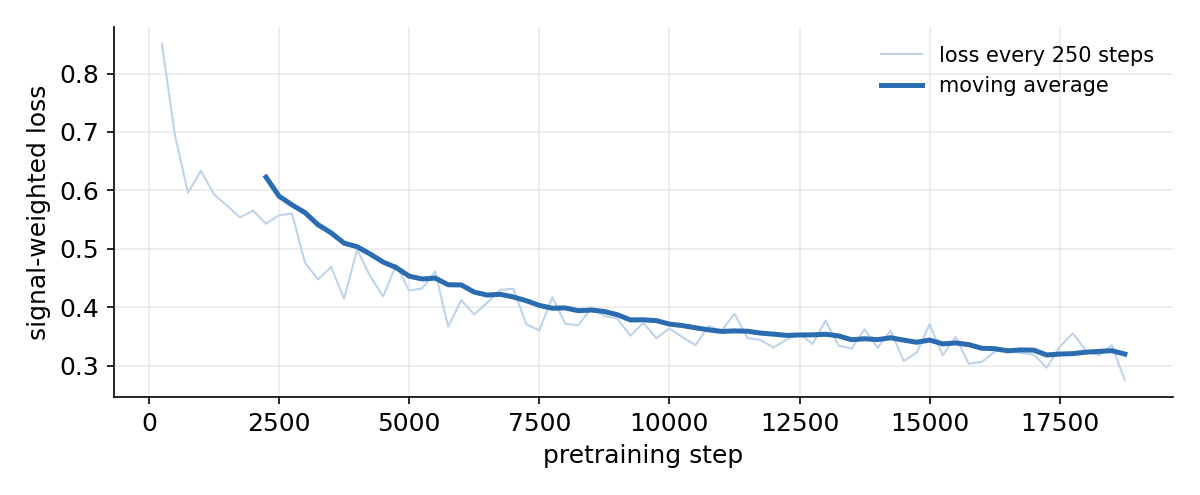
\includegraphics[width=0.62\linewidth]{fig/ssl_v2_loss.png}
\caption{Pretraining loss (Eq.~\ref{eq:ssl}) over 19k steps on an 8\,GB laptop GPU.}
\label{fig:sslloss}
\end{figure}

\subsection{Fine-tuning (recipe E)}
\label{sec:recipe}
Networks are initialised from the SSL checkpoint except the output convolutions and trained with Dice\,+\,BCE on the 82 annotated patches: SGD with Nesterov momentum 0.99, learning rate $10^{-2}$ with polynomial decay, weight decay $3\cdot10^{-5}$, batch 2, 250 iterations per epoch; 33\% of crops are centred on foreground and structure types are sampled \emph{uniformly} so that the six types contribute equally regardless of how many volumes or voxels they have. Weights are averaged with an exponential moving average (decay 0.999) \cite{tarvainen2017meanteacher}. Augmentation comprises flips and $90^\circ$ rotations, zoom (0.75--1.35), small rotations, smooth bias fields, low-resolution simulation, blur, and brightness, contrast, gamma and noise perturbations. The learning-rate schedule is tied to a wall-clock deadline, so an interrupted run resumes with a compressed schedule rather than overrunning. This recipe was chosen on the leave-family-out proxy (Section~\ref{sec:validation}); it replaced an earlier recipe with percentile normalisation and AdamW (v11).

\paragraph{Ensemble members.} v15a ($96^3$, 73 volumes with 9 held out, 174 epochs) and v15b ($96^3$, all 82 volumes, 187 epochs) were trained on one NVIDIA RTX~4060 Laptop GPU (8\,GB). The two contiguous experts used by the routed entry ($128^3$ patches, all 82 volumes, about 50 epochs each) were trained with the same recipe and initialisation on an NVIDIA A100 (40\,GB).

\subsection{Inference}
Volumes are z-score normalised as above and segmented with a Gaussian-weighted sliding window (50\% overlap) and four-flip test-time augmentation (identity and one flip per axis), averaged over the ensemble. Planes that are entirely zero (padding) are masked. The probability map is thresholded at 0.45 and components smaller than 4 voxels are removed. A foreground-density probe recognises sparse plaque-like volumes and applies a stricter profile (threshold 0.30, components $\geq 8$ voxels). Finally, connected components are relabelled so that the evaluation library's instance matching is well defined. This is the complete Task~2 entry (``v15'').

\subsection{Routed entry: morphology router and foreground anchoring}
\label{sec:routing}
On the leave-family-out proxy, $128^3$ context improved the unseen nerve family by about $+0.07$ Dice and clDice but cost a similar amount on unseen cells (Table~\ref{tab:ssl}), so a single patch size is not best for both categories. Because the category of a test volume is not given, the Task~1 entry infers it from v15's own mask $B=\{p_{15}>0.45\}$. Over the connected components of $B$ with at least 20 voxels (SimpleITK shape statistics \cite{lowekamp2013simpleitk}), a volume is \emph{contiguous} if one component dominates (largest component $\geq$ 30\% of the foreground with at most 1,000 components) or if objects are elongated (size-weighted mean principal-axis elongation $\geq$ 3); volumes with less than 0.05\% foreground (plaque-like) stay isolated (Fig.~\ref{fig:router}).

For a contiguous volume the probability is blended, $p=\tfrac12 p_{15}+\tfrac12 p_{128}$, where $p_{128}$ averages the two $128^3$ experts (one pass each, without flip augmentation, to respect the per-case time limit). The threshold is then \emph{anchored} per volume so that the result contains as much foreground as v15:
\begin{equation}
t^\star=\mathrm{clip}\Big(Q_{1-f}\big(p\,|\,\Omega\big),\;0.05,\;0.95\Big),\qquad f=\frac{|\{x\in\Omega:\,p_{15}(x)>0.45\}|}{|\Omega|},
\label{eq:anchor}
\end{equation}
where $\Omega$ are the non-padding voxels and $Q_q$ the $q$-quantile. The experts therefore decide \emph{which} voxels are foreground and v15 decides \emph{how many}. Anchoring is motivated by the calibration findings of Section~\ref{sec:calibration}; isolated volumes follow the v15 path unchanged, so the two entries produce identical isolated predictions.

\begin{figure}[!htbp]
\centering
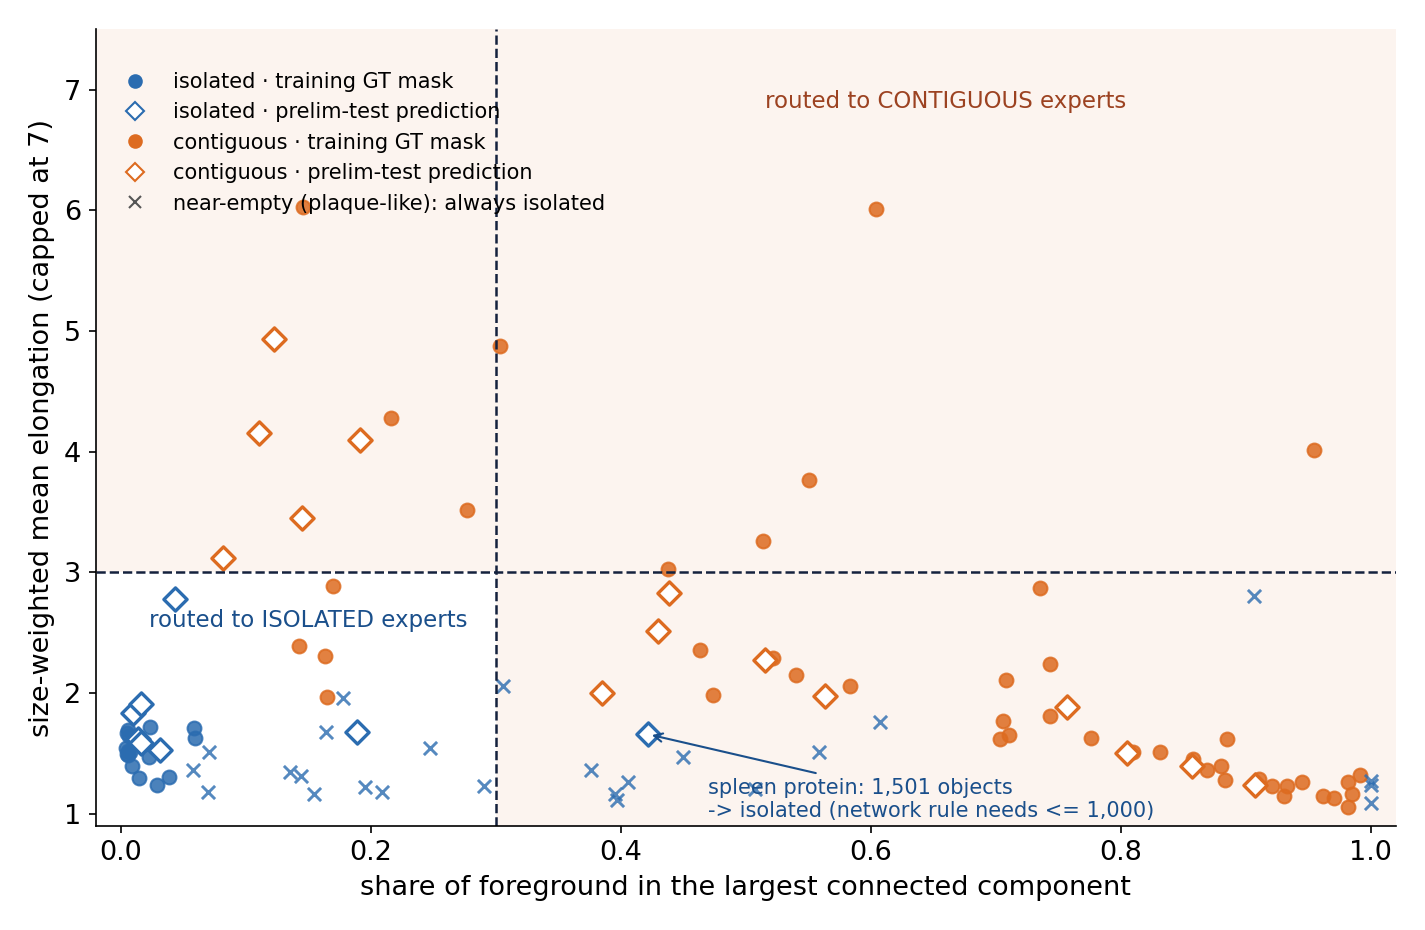
\includegraphics[width=0.78\linewidth]{fig/router_space.png}
\caption{Router features for 82 training masks and 26 preliminary-test predictions. All 26 preliminary-test volumes are routed correctly. On all 108 volumes the rule makes 4 errors, all contiguous volumes kept on the isolated path (which reproduces v15); re-fitting the thresholds without each held-out structure type (11 types) gives 5 errors, one of them an isolated volume sent to the experts, and returns the shipped thresholds in 10 of 11 folds.}
\label{fig:router}
\end{figure}

\begin{table}[!htbp]
\centering\small
\caption{Settings of the submitted models.}
\label{tab:settings}
\begin{tabular}{p{0.2\linewidth}p{0.74\linewidth}}
\toprule
Component & Setting \\
\midrule
SSL & 3,400 unannotated patches; $96^3$ crops (50\% signal-centred); $12^3$ block masks over 50--75\%; structure-weighted Huber loss (Eq.~\ref{eq:ssl}); AdamW $3\cdot10^{-4}$, cosine; batch 2; 18,978 steps \\
Architecture & DynUNet, 5 levels, filters 32/64/128/256/320, residual blocks, instance norm, deep supervision; 16.7\,M parameters \\
Fine-tuning & z-score $[-3,25]$; SGD Nesterov 0.99, lr $10^{-2}$ poly, wd $3\cdot10^{-5}$; Dice\,+\,BCE; 33\% foreground crops; uniform type sampling; EMA 0.999; batch 2; 250 it./epoch \\
v15 (Task 2) & v15a + v15b ($96^3$); sliding window, overlap 0.5, 4-flip TTA; threshold 0.45, components $\geq 4$; plaque profile 0.30 / $\geq 8$ \\
Routed (Task 1) & v15 path for isolated volumes; contiguous volumes: $\tfrac12$v15 + $\tfrac12$(two $128^3$ experts, single pass), anchored threshold (Eq.~\ref{eq:anchor}) \\
Hardware & SSL and v15: RTX 4060 Laptop (8\,GB); $128^3$ experts: A100 (40\,GB); inference: T4 (16\,GB) \\
\bottomrule
\end{tabular}
\end{table}

% ------------------------------------------------------------------------------------------
\section{Validating for unseen structure types}
\label{sec:validation}

\paragraph{Held-out split.} Nine annotated volumes (3 plaques, 1 nuclei, 1 c-Fos, 2 vessels, 1 peripheral nerve, 1 axon) were held out from v15a and from the development models. This split measures accuracy on new volumes of \emph{seen} types.

\paragraph{Leave-family-out proxy.} To imitate the test set's unseen types we trained models without any c-Fos or peripheral-nerve volume and scored exactly those (9 c-Fos volumes with Dice/PQ, 6 nerve volumes with Dice/clDice). c-Fos stands in for unseen cell types (microglia, organ proteins) and peripheral nerves for unseen fibre networks (gut nerve, lymphatics). The fine-tuning recipe, the pretraining variant and the per-category patch size were chosen on this proxy.

\paragraph{Label-free unseen-type calibration.} For each candidate we measured the fraction of voxels it segments on the \emph{unlabelled} preliminary-test volumes, per structure type, relative to a reference model (v15). This needs no labels and no submission.

% ------------------------------------------------------------------------------------------
\section{Results}

\subsection{Final test phase}

\begin{table}[!htbp]
\centering\small
\caption{Final-test metrics of our two entries (mean\,$\pm$\,s.d.\ over test volumes).}
\label{tab:final}
\resizebox{\linewidth}{!}{%
\begin{tabular}{llcccc}
\toprule
Task & Entry & isolated DSC & isolated PQ & contiguous DSC & contiguous clDice \\
\midrule
Task 1 (fixed data) & Routed + anchored & $0.547\pm0.262$ & $0.360\pm0.242$ & $0.653\pm0.155$ & $0.738\pm0.152$ \\
Task 2 (open data) & v15 & $0.547\pm0.262$ & $0.360\pm0.242$ & $0.653\pm0.155$ & $0.737\pm0.153$ \\
\bottomrule
\end{tabular}}
\end{table}

\begin{figure}[!htbp]
\centering
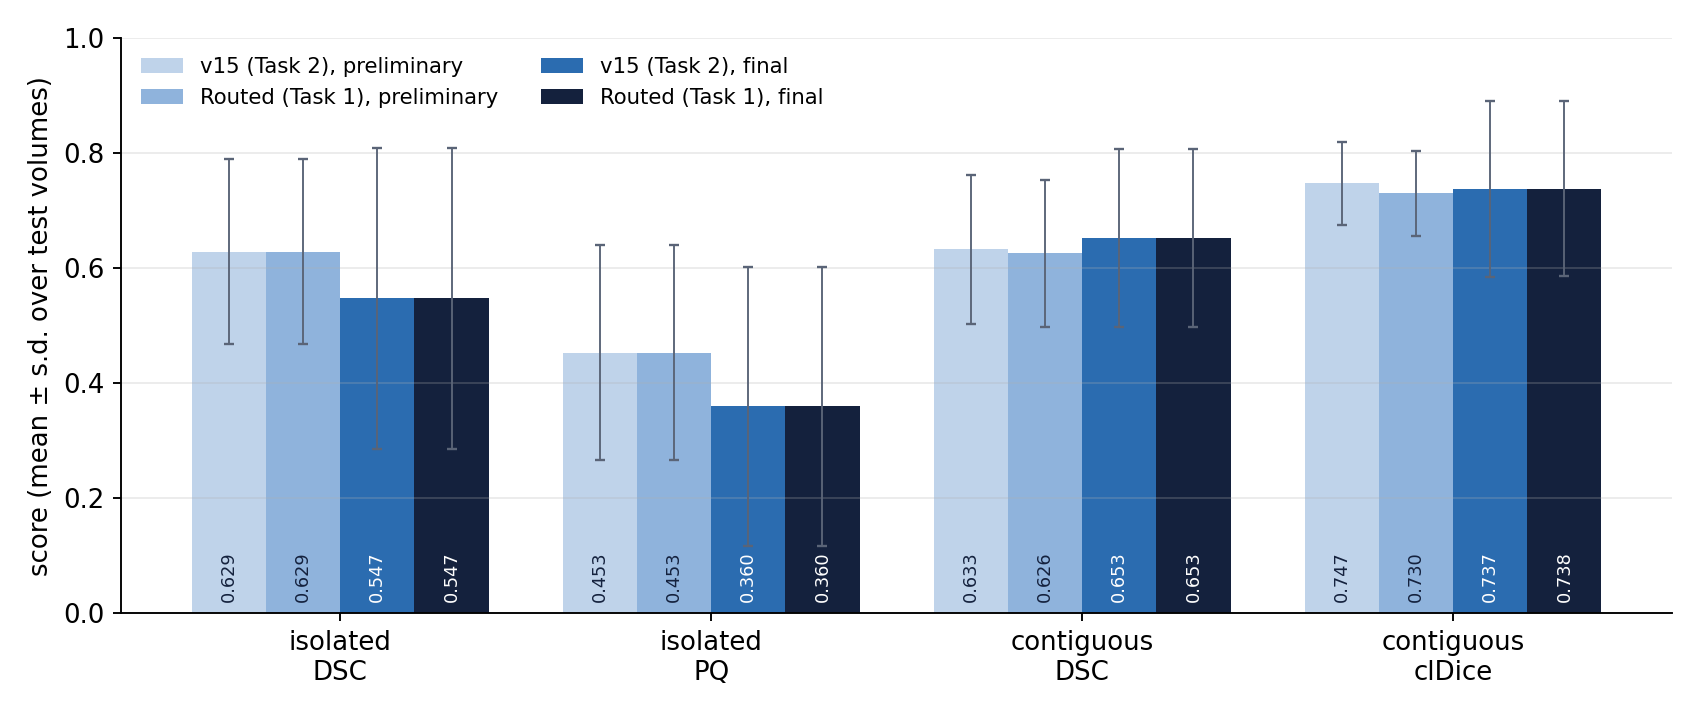
\includegraphics[width=0.92\linewidth]{fig/final_metrics.png}
\caption{Our metrics on the preliminary and final test sets (mean\,$\pm$\,s.d.\ over test volumes). Isolated results are identical for the two entries by construction.}
\label{fig:final}
\end{figure}

Table~\ref{tab:final} and Fig.~\ref{fig:final} give our final-test results. On contiguous structures the entries reached Dice 0.653 and clDice 0.737--0.738 with a standard deviation across volumes of about 0.15, that is, few contiguous volumes on which the segmentation failed. On isolated structures they reached Dice 0.547 and PQ 0.360; compared with the preliminary test, isolated scores fell (0.629/0.453 $\to$ 0.547/0.360) while contiguous Dice rose (0.633 $\to$ 0.653). The two entries are identical on isolated volumes by construction and differ on contiguous volumes by $+0.0001$ Dice and $+0.0008$ clDice in favour of the routed variant (Table~\ref{tab:prelimfinal}).

\begin{table}[!htbp]
\centering\small
\caption{Our entries on the preliminary (26 volumes) and final test sets. Isolated predictions are identical; routing changes only contiguous volumes.}
\label{tab:prelimfinal}
\begin{tabular}{llccccc}
\toprule
Phase & Entry & iso DSC & iso PQ & cont DSC & cont clDice & mean \\
\midrule
\multirow{3}{*}{Preliminary} & v15 (Task 2) & 0.629 & 0.453 & 0.633 & 0.747 & 0.616 \\
 & Routed (Task 1) & 0.629 & 0.453 & 0.626 & 0.730 & 0.610 \\
 & difference & 0 & 0 & $-0.007$ & $-0.017$ & $-0.006$ \\
\midrule
\multirow{3}{*}{Final} & v15 (Task 2) & 0.547 & 0.360 & 0.653 & 0.737 & 0.574 \\
 & Routed (Task 1) & 0.547 & 0.360 & 0.653 & 0.738 & 0.575 \\
 & difference & 0 & 0 & $+0.000$ & $+0.001$ & $+0.000$ \\
\bottomrule
\end{tabular}
\end{table}

\subsection{Qualitative results}
Fig.~\ref{fig:qualhold} shows v15a on held-out volumes it never saw during training; Fig.~\ref{fig:qualunseen} shows v15 on preliminary-test volumes of structure types that have no annotated example. Unseen fibre networks (gut nerve, lymphatic vessels) are traced as connected networks, which is consistent with the strong contiguous scores; on unseen cell types the bright cells are detected, but the proxy analysis of Section~\ref{sec:cfos} shows that dim cells are missed and detected cells are under-sized, which is where the remaining gap lies. (Slab projections overlay all predictions within the slab, so adjacent objects can appear joined.)

\begin{figure}[!htbp]
\centering
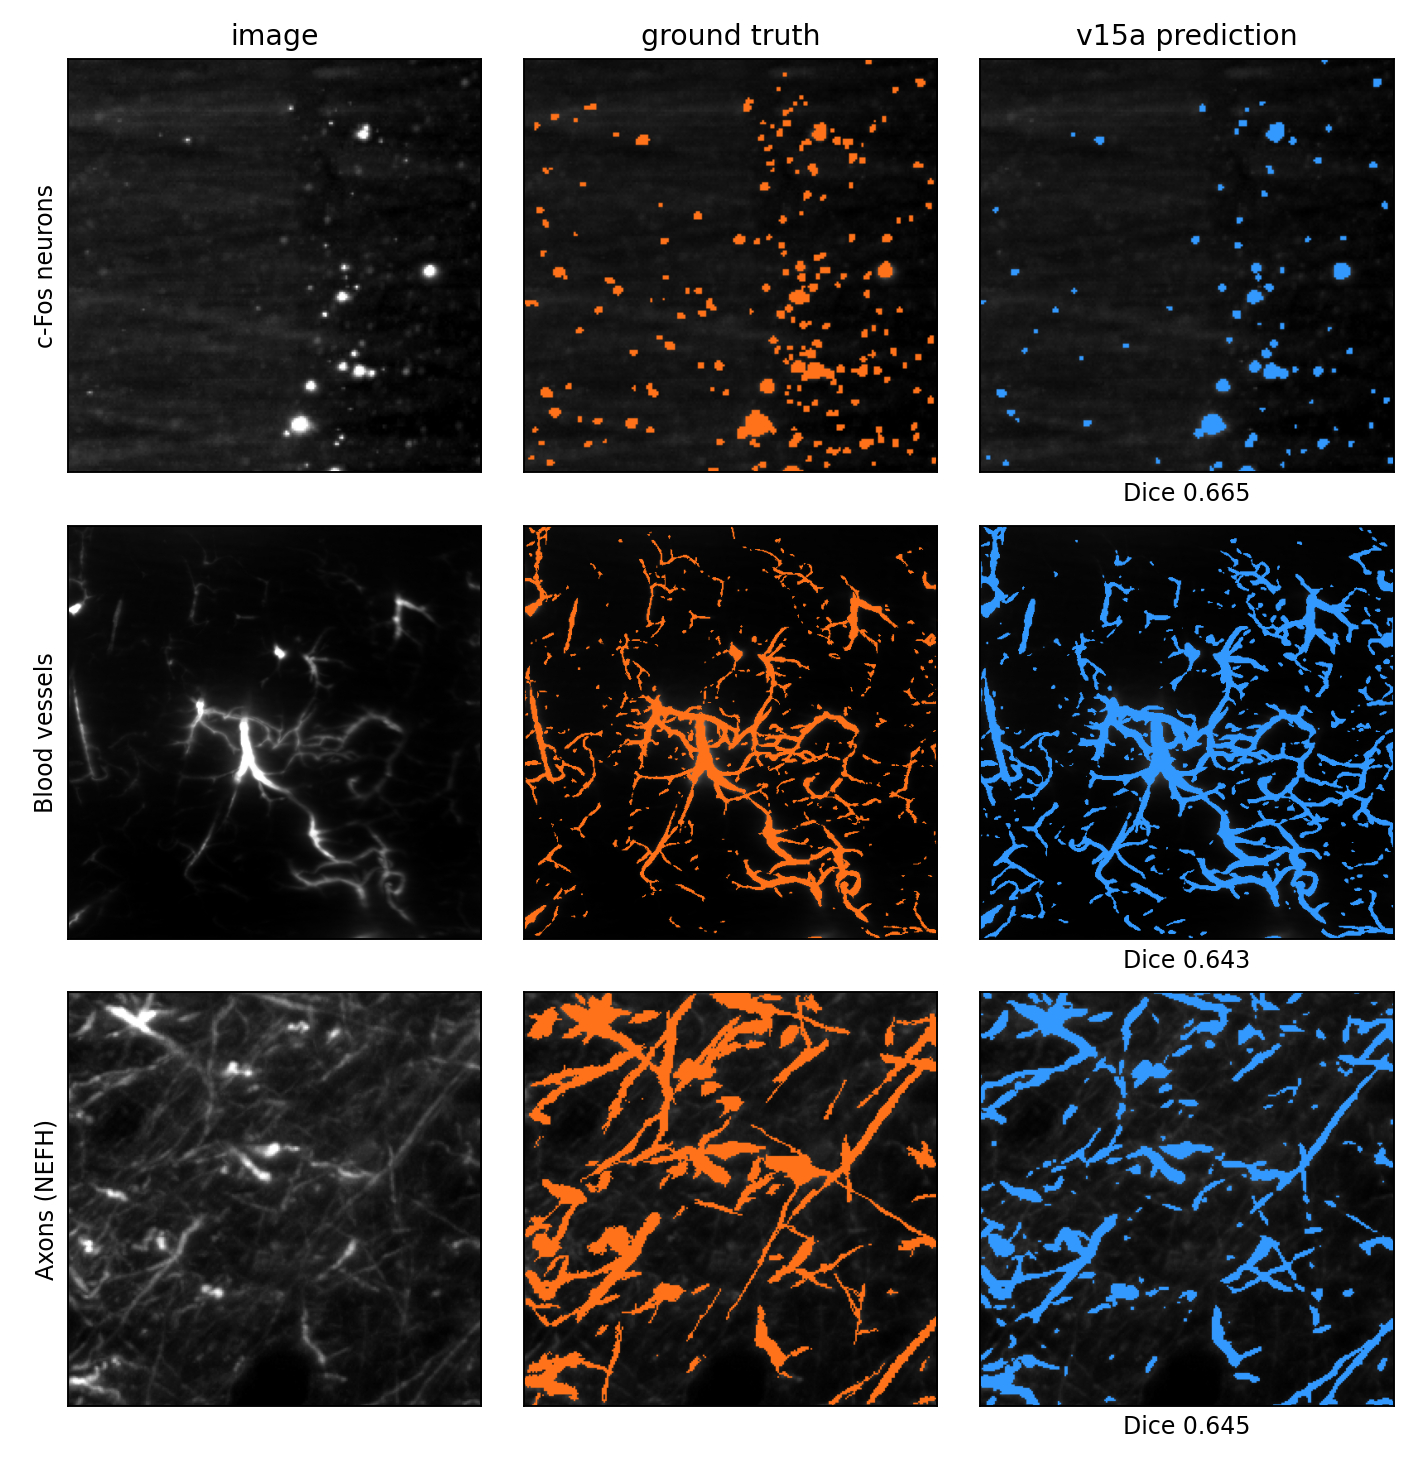
\includegraphics[width=0.74\linewidth]{fig/qual_holdout.png}
\caption{v15a on held-out volumes of seen types (slab projections; Dice on the full volume).}
\label{fig:qualhold}
\end{figure}

\begin{figure}[!htbp]
\centering
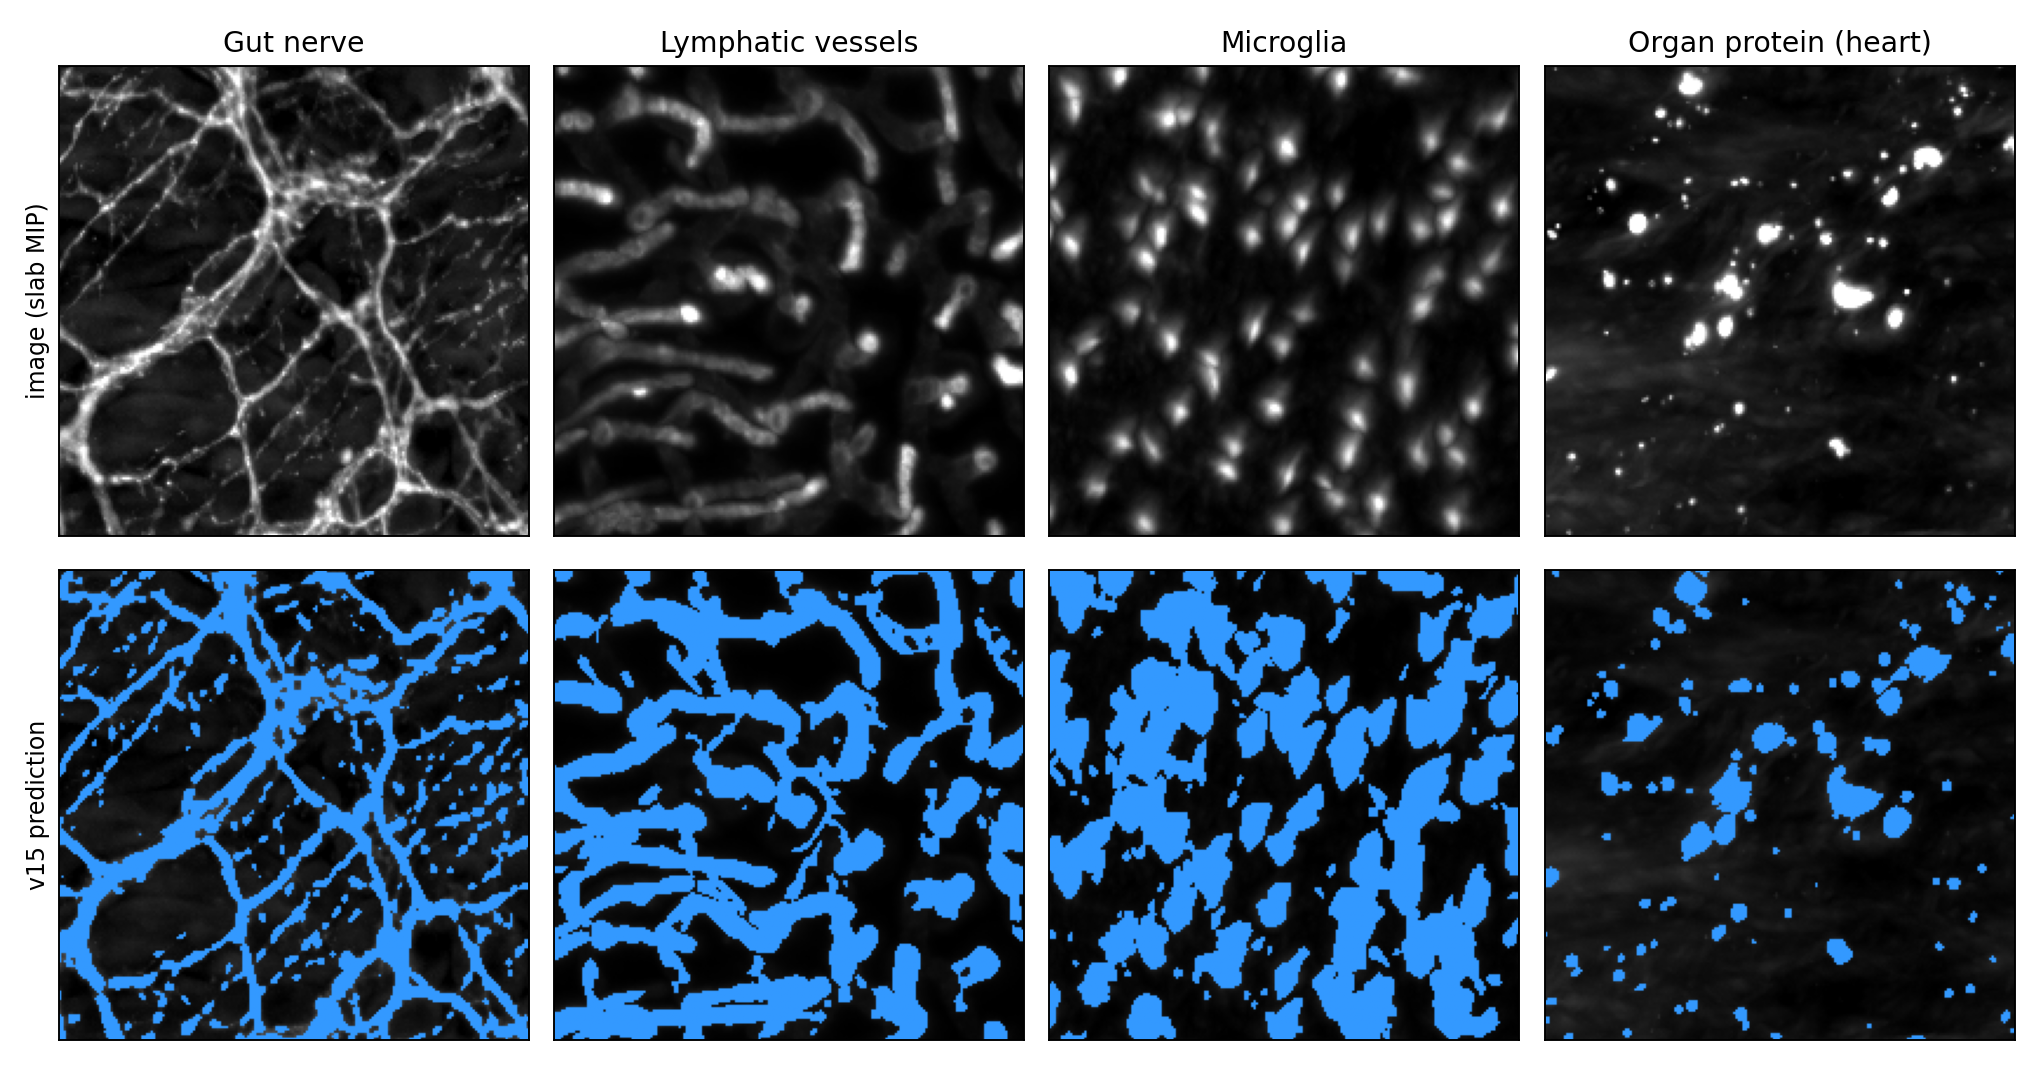
\includegraphics[width=\linewidth]{fig/qual_unseen.png}
\caption{v15 on preliminary-test volumes of structure types with no annotated example (no labels available). Projections over a 40-slice slab centred on the densest part of the prediction.}
\label{fig:qualunseen}
\end{figure}

\subsection{Held-out accuracy did not predict the preliminary-test score}
\label{sec:calibration}

\begin{table}[!htbp]
\centering\small
\caption{Development history. Held-out: 9 volumes of seen types (thresholds tuned per model). Prelim.\ test: mean of the four metrics on the 26 preliminary-test volumes. Foreground ratio: fraction of voxels segmented on unlabelled test volumes relative to v15.}
\label{tab:history}
\begin{tabular}{lp{0.3\linewidth}ccccc}
\toprule
Model & Change & held-out & prelim.\ test & fg.\ seen types & fg.\ unseen types \\
\midrule
v11 & percentile norm., AdamW & 0.640 & 0.537 & \x0.96 & \x1.19 \\
\textbf{v15} & recipe E (proxy-selected) + SSL (Sec.~\ref{sec:ssl}) & 0.658 & \textbf{0.616} & \x1.00 & \x1.00 \\
v17 & geometry-completion SSL, slowed encoder, $112^3$ & \textbf{0.671} & 0.573 & \x1.03 & \x0.75 \\
\bottomrule
\end{tabular}
\end{table}

\begin{figure}[!htbp]
\centering
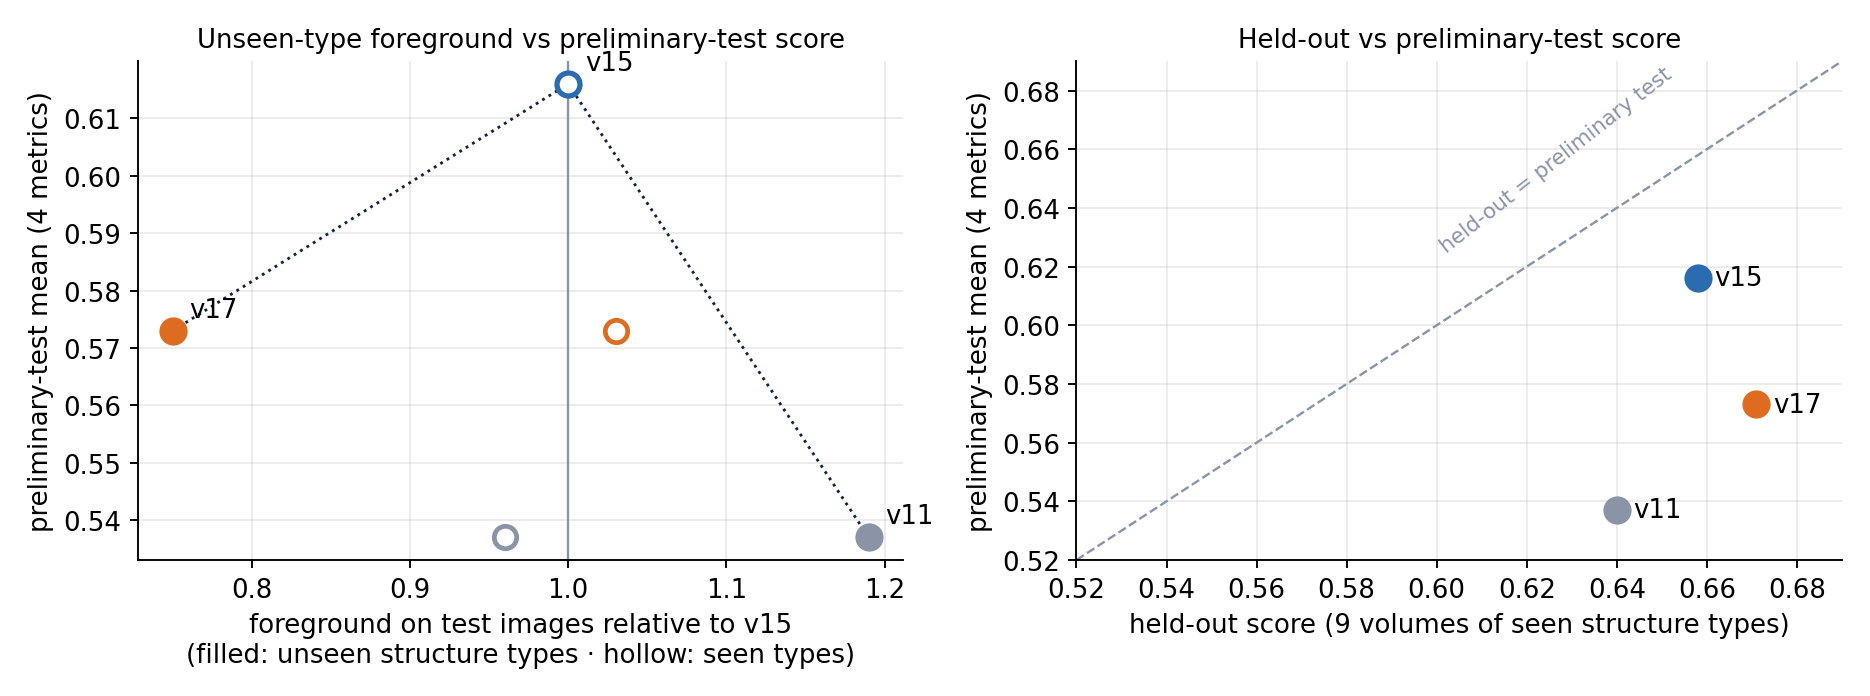
\includegraphics[width=\linewidth]{fig/calibration_prelim.png}
\caption{Left: preliminary-test mean against foreground on unseen (filled) and seen (hollow) structure types relative to v15. Right: held-out score against preliminary-test score; v17 is higher than v15 on the held-out split and lower on the preliminary test.}
\label{fig:calib}
\end{figure}

Table~\ref{tab:history} and Fig.~\ref{fig:calib} trace our three scored models. Replacing the v11 recipe by the proxy-selected recipe E raised the preliminary-test mean by $+0.079$ (isolated Dice $+0.130$, PQ $+0.171$) while the held-out score moved by only $+0.018$. A later model, v17, used a geometry-completion pretext task \cite{frangi1998vesselness}, a slowed encoder with a heads-first warm-up \cite{kumar2022lpft} and $112^3$ patches; it scored highest of the three on the held-out split (0.671 vs.\ 0.658) but 0.043 lower on the preliminary test. On seen types all three models segment within 4\% of each other. On unseen types they diverge: v11 segments 19\% more than v15 (microglia \x1.56, gut nerve \x1.54) and v17 25\% less (microglia \x0.55, gut nerve \x0.67, lymphatic vessels \x0.73), and the preliminary-test score falls whichever way a model departs from v15. With three scored models this is a case study rather than a fitted relation, but it gave us a label-free gate: after v17 we rejected any candidate whose unseen-type foreground departed markedly from v15's.

The same gate explains the design of the routed entry (Fig.~\ref{fig:fgratio}). Without anchoring, routing contiguous volumes to the $128^3$ experts under-segmented the unseen contiguous types (gut nerve and lymphatic vessels \x0.83; \x0.87--0.90 when blended with v15)---the direction that had cost v17. With anchoring (Eq.~\ref{eq:anchor}) every type stays within \x0.99--1.01, and on the four held-out contiguous volumes the anchored blend matched v15 (Dice/clDice 0.752/0.816 vs.\ 0.753/0.814; Table~\ref{tab:holdout}).

\begin{figure}[!htbp]
\centering
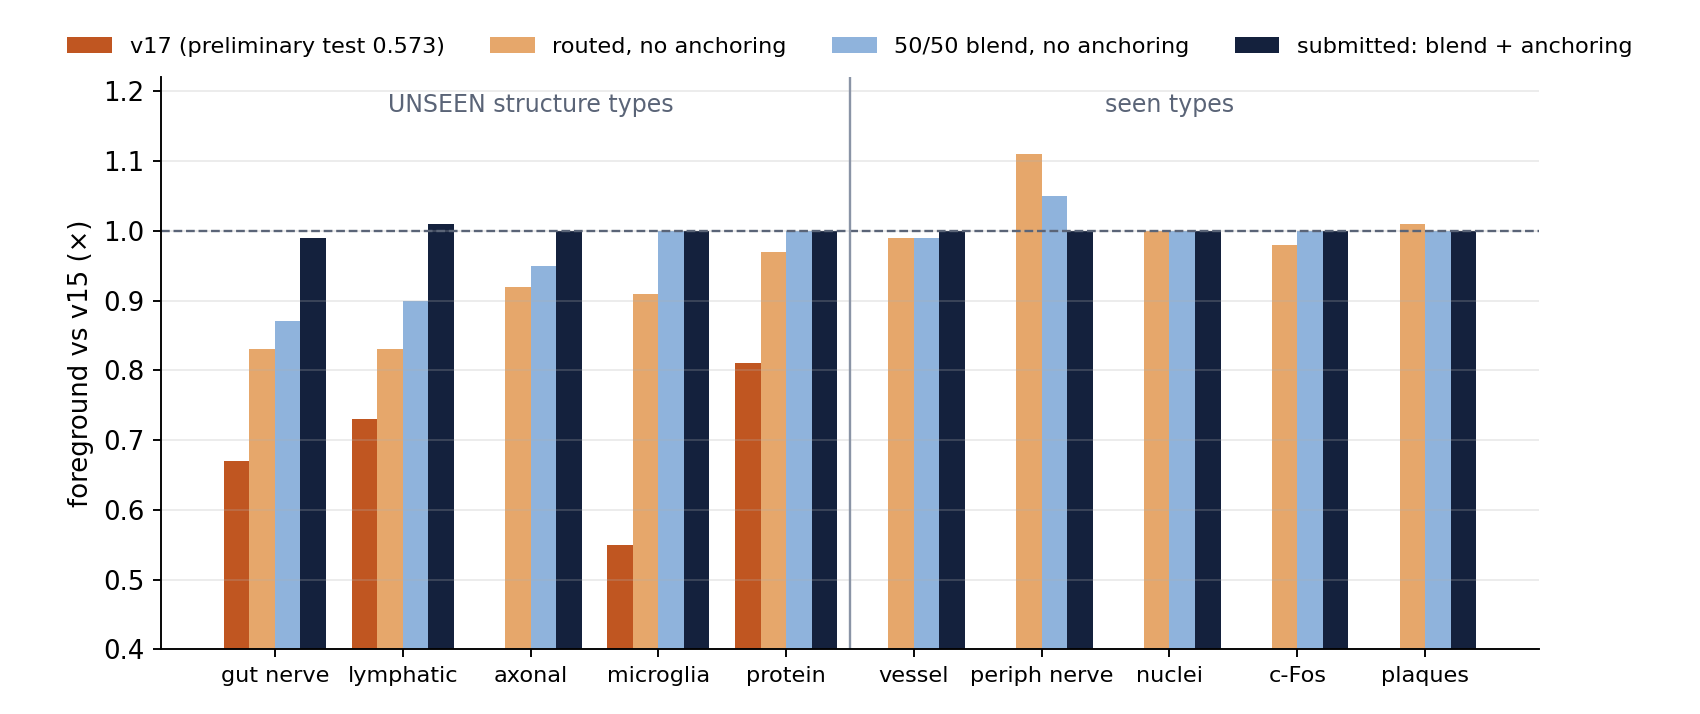
\includegraphics[width=\linewidth]{fig/fg_ratio_candidates.png}
\caption{Foreground relative to v15 on the unlabelled preliminary-test volumes, by structure type. All three routed candidates routed 26/26 volumes correctly.}
\label{fig:fgratio}
\end{figure}

\begin{table}[!htbp]
\centering\small
\caption{Contiguous held-out volumes (4) with models that never saw them: v15a and a $128^3$ expert trained without the held-out split.}
\label{tab:holdout}
\begin{tabular}{lccc}
\toprule
Contiguous route & Dice & clDice & mean \\
\midrule
v15a alone, threshold 0.45 & 0.753 & 0.814 & 0.783 \\
$128^3$ expert alone, best threshold (0.65) & 0.749 & 0.809 & 0.779 \\
50/50 blend, best fixed threshold (0.55) & 0.756 & 0.817 & 0.787 \\
50/50 blend, anchored threshold (submitted) & 0.752 & 0.816 & 0.784 \\
\bottomrule
\end{tabular}
\end{table}

\subsection{Pretraining and context on the leave-family-out proxy}

\begin{table}[!htbp]
\centering\small
\caption{Leave-family-out proxy: c-Fos and peripheral nerves never used for fine-tuning. Best checkpoint of each run on the proxy, so absolute values are optimistic; comparisons are like for like.}
\label{tab:ssl}
\begin{tabular}{lcccc}
\toprule
Pretraining and patch size & score & c-Fos Dice / PQ & nerve Dice / clDice \\
\midrule
Signal-weighted reconstruction (ours), $96^3$ & \textbf{0.387} & \textbf{0.499 / 0.221} & 0.436 / 0.390 \\
Signal-weighted reconstruction (ours), $128^3$ & \textbf{0.387} & 0.431 / 0.152 & \textbf{0.507 / 0.457} \\
Geometry completion, $96^3$ & 0.335 & 0.371 / 0.124 & 0.442 / 0.402 \\
Geometry completion, $112^3$, slowed encoder & 0.377 & 0.420 / 0.142 & 0.493 / 0.453 \\
\bottomrule
\end{tabular}
\end{table}

Table~\ref{tab:ssl} compares pretext tasks and context sizes on the proxy. Signal-weighted reconstruction was the best pretraining we tried; a geometry-completion task that predicts distance-to-signal and Hessian-based tube and blob fields was worse on unseen cells. Larger context improves the unseen nerve family by about $+0.07$ on both Dice and clDice and costs a similar amount on unseen cells---the observation behind routing. Against training from scratch at matched progress the proxy difference was small (0.352 vs.\ 0.350), so we do not claim a large benefit of pretraining at our scale (19k steps at batch 2).

\subsection{The late-training decline on unseen types is miscalibration, not forgetting}

\begin{figure}[!htbp]
\centering
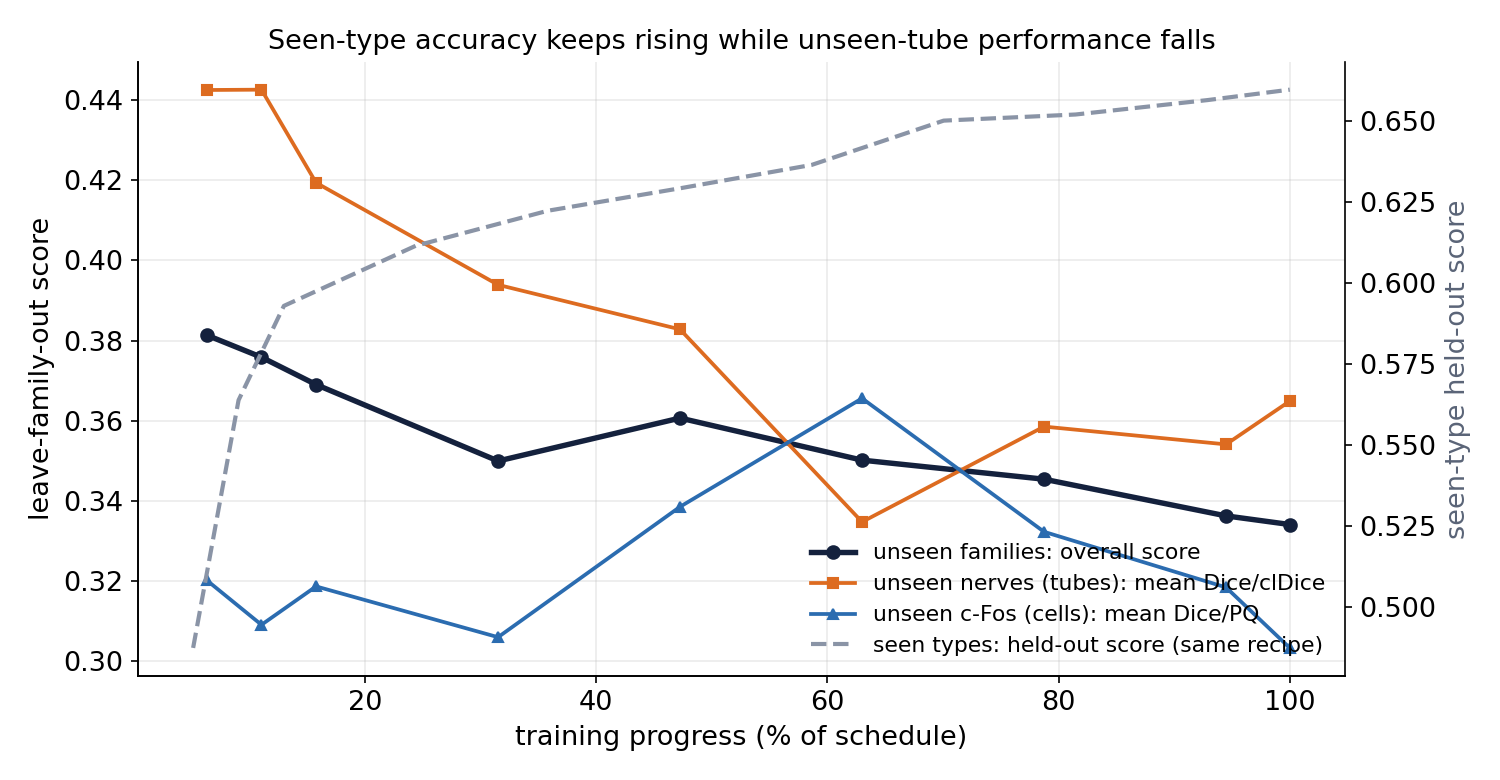
\includegraphics[width=0.9\linewidth]{fig/generalisation_curve.png}
\caption{Leave-family-out score of one training run by snapshot (best of four thresholds per snapshot) and the seen-type held-out score of the same recipe. Seen-type accuracy rises from 0.49 to 0.66 while the unseen score peaks at the first snapshot (0.381) and ends 12\% lower (0.334), driven by the unseen nerve family.}
\label{fig:curve}
\end{figure}

\begin{figure}[!htbp]
\centering
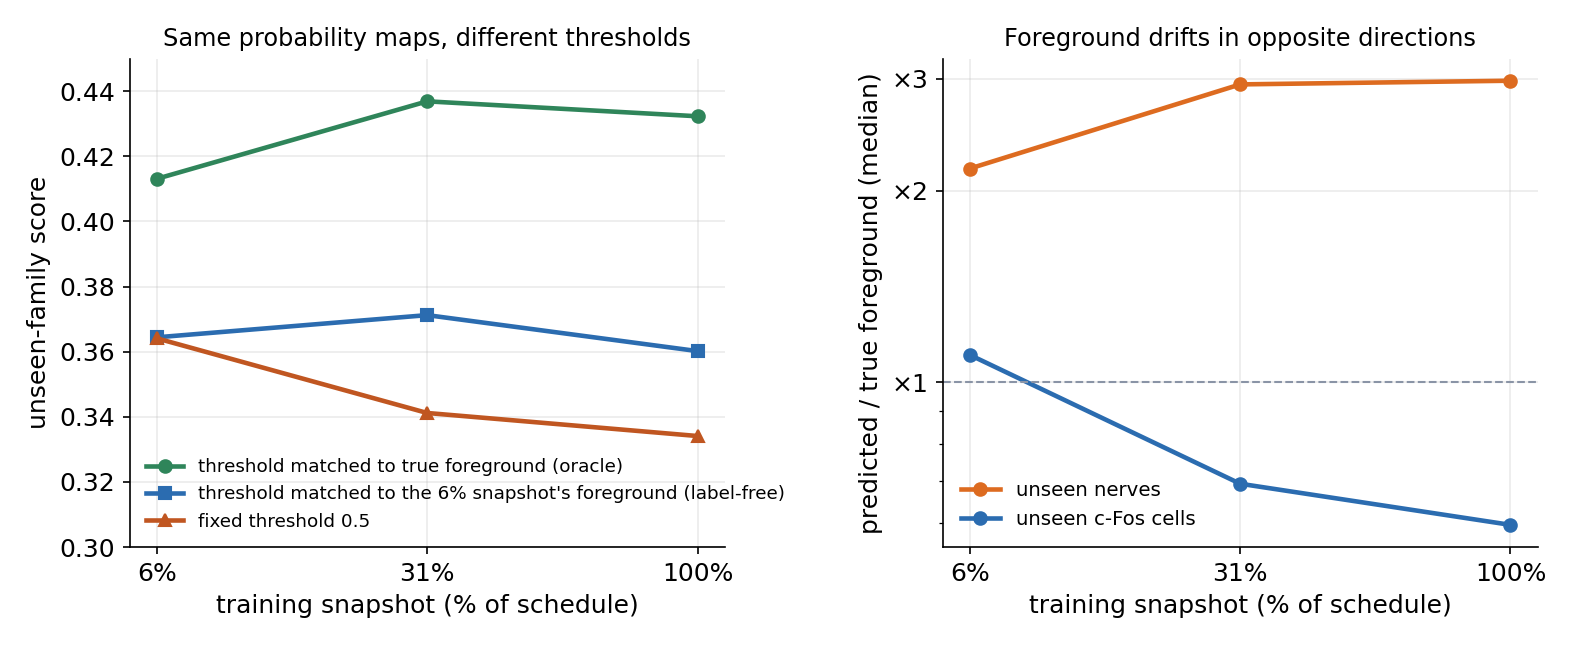
\includegraphics[width=\linewidth]{fig/calibration_drift.png}
\caption{Left: the same probability maps scored with a fixed threshold, with a per-volume threshold matching the early snapshot's foreground (label-free), and with a per-volume threshold matching the true foreground (oracle). Right: median ratio of predicted to true foreground on the two withheld families.}
\label{fig:drift}
\end{figure}

On the withheld families the proxy score peaked at the first evaluated snapshot and fell by 12\% by the end of training, while the seen-type score kept rising (Fig.~\ref{fig:curve}). To test whether the network forgets how to recognise unseen structures or merely mis-sizes them, we re-scored three snapshots (6\%, 31\% and 100\% of training) on identical probability maps with different thresholding rules (Fig.~\ref{fig:drift}, Table~\ref{tab:drift}).

\begin{table}[!htbp]
\centering\small
\caption{Unseen-family score of three snapshots of one run under different thresholding rules, and the predicted-to-true foreground ratio (median over volumes).}
\label{tab:drift}
\resizebox{\linewidth}{!}{%
\begin{tabular}{lccccc}
\toprule
Snapshot & fixed 0.5 & anchored to 6\% snapshot & matched to truth (oracle) & fg.\ nerves / cells & threshold matching truth \\
\midrule
6\% & 0.364 & 0.364 & 0.413 & \x2.17 / \x1.10 & 0.86 / 0.57 \\
31\% & 0.341 & \textbf{0.371} & \textbf{0.437} & \x2.94 / \x0.69 & 0.94 / 0.34 \\
100\% & 0.334 & 0.360 & 0.432 & \x2.98 / \x0.60 & 0.975 / 0.09 \\
\bottomrule
\end{tabular}}
\end{table}

Given the true amount of foreground, the fully trained model scores \emph{higher} than the early snapshot (0.432 vs.\ 0.413): its separation of foreground from background keeps improving. What degrades is calibration, and in opposite directions for the two unseen families: tubes become over-segmented (\x2.2 $\to$ \x3.0 of the true foreground) and cells under-segmented (\x1.10 $\to$ \x0.60), so that the thresholds matching the truth move to 0.975 and 0.09. No single global threshold can undo drift in opposite directions, which is why threshold sweeps barely changed the curve in Fig.~\ref{fig:curve}. Choosing each volume's threshold so that the late snapshot segments as much as the early one---without labels---recovers most of the loss ($0.334\to0.360$), and the anchored mid-training snapshot (0.371) is better than either ingredient alone. Foreground anchoring in the routed entry applies the same principle with v15 as the reference.

\subsection{Test-time self-training reverses sign with topology}

\begin{figure}[!htbp]
\centering
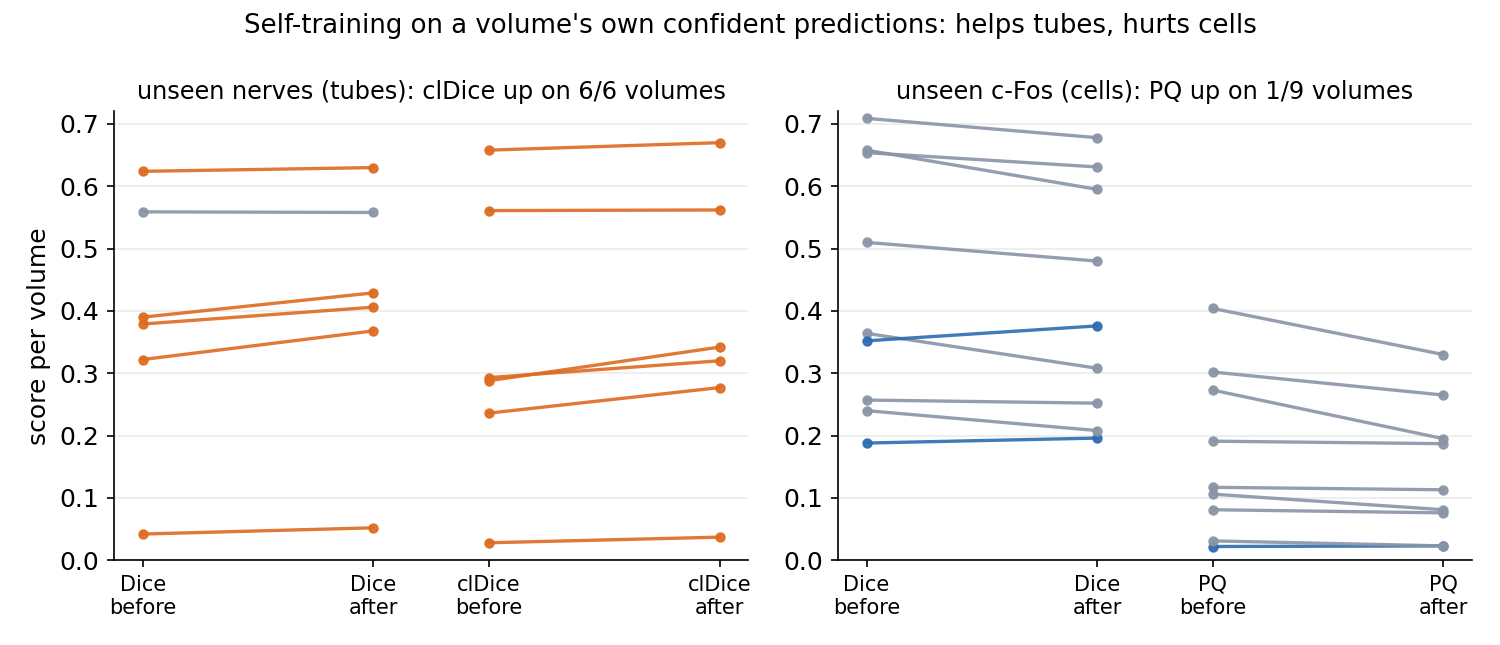
\includegraphics[width=0.9\linewidth]{fig/ttt_split.png}
\caption{Per-volume effect of test-time self-training on the withheld families (end-of-training model, threshold 0.6). Coloured: improved; grey: worse.}
\label{fig:ttt}
\end{figure}

We adapted a copy of the model to each test volume for 40 SGD steps (learning rate $10^{-3}$) on its own confident predictions: voxels above 0.85 are foreground targets, voxels below 0.10 background and the rest are ignored (masked BCE\,+\,soft Dice) \cite{lee2013pseudolabel,sun2020ttt}. Applied to every volume the effect is nil (0.334 $\to$ 0.333). Split by structure class it is large and consistent in sign (Fig.~\ref{fig:ttt}): on unseen nerves Dice and clDice rise by $+0.033$ and $+0.042$ (clDice up on 6/6 volumes), on unseen cells Dice and PQ fall by $-0.041$ and $-0.038$ (PQ down on 8/9 volumes). Restricted to contiguous volumes by the router, the proxy score rises to 0.353. Along a fibre the confident voxels form a connected core, and learning from them extends the prediction into fainter segments; for cells the confident voxels are the bright centres of cells already found, so self-training reinforces the existing under-sizing (Section~\ref{sec:cfos}). We did not submit this variant because it had not been validated on the $128^3$ experts and roughly doubles inference time on contiguous volumes.

\subsection{Why unseen cells score low on panoptic quality}
\label{sec:cfos}

\begin{figure}[!htbp]
\centering
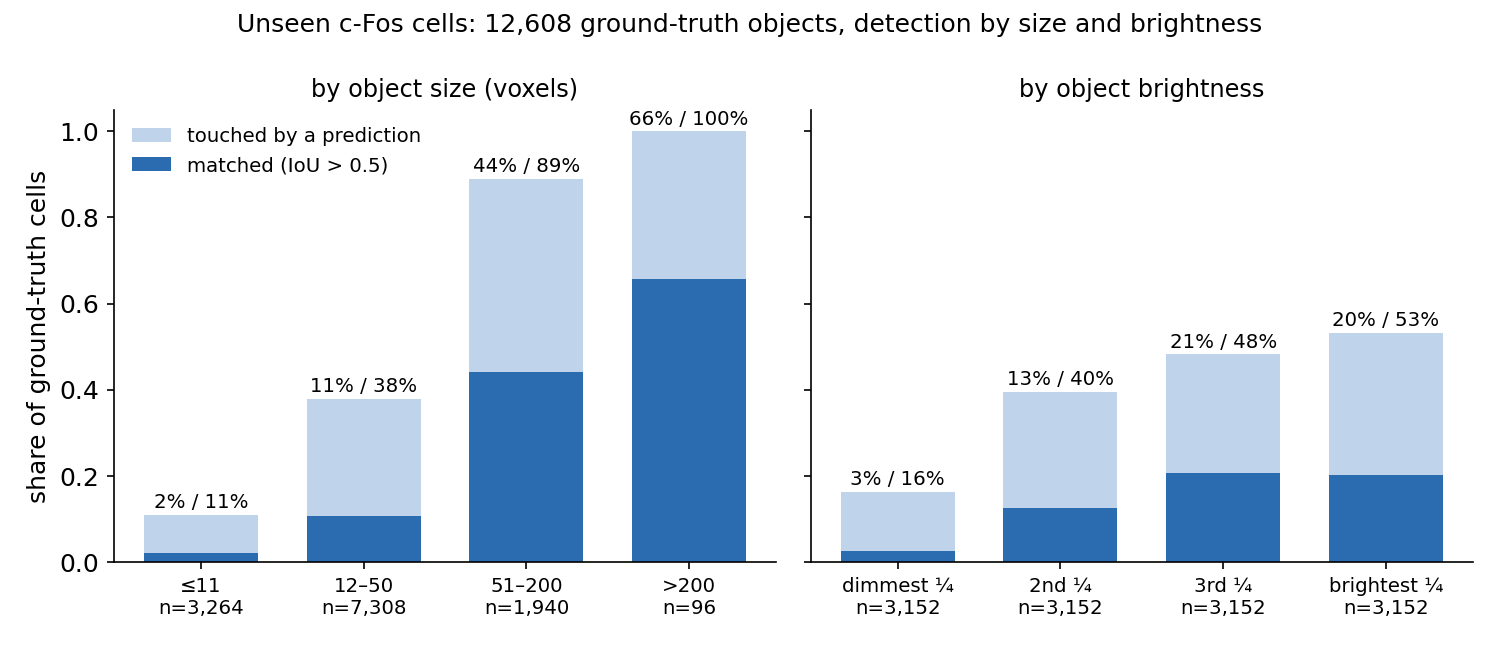
\includegraphics[width=0.9\linewidth]{fig/cfos_detection.png}
\caption{Ground-truth c-Fos cells of the withheld family (12,608 objects) that are touched by a prediction or matched at IoU\,$>$\,0.5, by object size and brightness.}
\label{fig:cfos}
\end{figure}

PQ counts a cell only if a predicted object overlaps it with IoU\,$>$\,0.5. Of the 12,608 ground-truth objects in the nine withheld c-Fos volumes, 39\% are touched by any prediction and 14\% matched; touched cells are predicted at a median of 0.50\x\ their true size; 26\% of the objects have at most 11 voxels (2\% matched); and the dimmest quarter is matched in 3\% of cases against 20\% for the brightest (Fig.~\ref{fig:cfos}). In the densest volumes the model predicts 505 objects against 1,401 annotated ones. The PQ gap on unseen cell types is therefore one of recall and size calibration, not of merged cells; consistent with this, splitting touching objects lowered PQ (Table~\ref{tab:neg}), and isolated structures remained our weakest category on the final test.

\subsection{Negative results}

\begin{table}[!htbp]
\centering\small
\caption{Ideas that did not transfer to unseen structure types (leave-family-out proxy unless noted).}
\label{tab:neg}
\begin{tabular}{p{0.34\linewidth}p{0.6\linewidth}}
\toprule
Idea & Result \\
\midrule
Hysteresis thresholding & c-Fos PQ 0.193 $\to$ 0.232, but Dice and both nerve metrics fell; overall 0.380 $\to$ 0.369 at best \\
Seeded watershed growth of objects & c-Fos PQ $+0.009$; overall fell as growth deepened (0.365 $\to$ 0.343) \\
Splitting touching objects & dense-cell PQ fell at every setting (0.206 $\to$ 0.188--0.205): objects are missed, not merged \\
Probability\,$\times$\,intensity fusion, region-percentile rules & small nerve gains, c-Fos Dice collapses; no rule helped both families \\
Multi-scale TTA (0.8/1.0/1.25) & 0.252 vs.\ 0.256 single-scale \\
Snapshot and mixed-recipe ensembles & 0.351 / 0.348, below the best single snapshot (0.361); mixing pretraining variants also lowered held-out accuracy \\
Router on image tubularity (Hessian) & 22/108 volumes misrouted; replaced by the mask-shape router \\
Test-time self-training on every volume & net zero: $+0.04$ on tubes cancelled by $-0.04$ on cells \\
Routed $128^3$ experts without anchoring & unseen contiguous foreground \x0.83--0.90 of v15 (Fig.~\ref{fig:fgratio}) \\
Routing with anchoring (submitted, Task 1) & $-0.006$ preliminary, $+0.000$ final vs.\ v15 (Table~\ref{tab:prelimfinal}) \\
\bottomrule
\end{tabular}
\end{table}

Table~\ref{tab:neg} lists the variants that did not help. Two patterns stand out. Post-processing that trades recall for object quality (hysteresis, watershed growth, object splitting) moved c-Fos PQ and nerve metrics in opposite directions, so no setting helped both. And every change that altered the amount of foreground on unseen types---in either direction---lost more than it gained, including routing to larger-context experts, which only became neutral once its foreground was anchored.

% ------------------------------------------------------------------------------------------
\section{Discussion}

\paragraph{What drove the result.} Our strongest category, contiguous structures, came from the v15 ensemble itself: routing to $128^3$ experts with anchoring changed the final-test contiguous scores by less than 0.001. The decisive choices were upstream---a fine-tuning recipe with uniform type sampling selected on unseen families, and a model whose foreground on unseen types we had checked against a reference. The low spread of our contiguous scores suggests that the model rarely fails outright on a new fibre type, which is what a calibrated amount of foreground buys.

\paragraph{Validation for open-set segmentation.} When most test volumes show unseen structure types, a held-out split of annotated volumes is not a reliable model-selection signal: in our case it overestimated the preliminary-test score by 0.04--0.10 and favoured the weaker of our two best models. A leave-family-out proxy and a label-free foreground check were cheap to add and would have prevented our one clearly worse submission. The proxy experiment adds a mechanism: longer training keeps improving voxel-level discrimination on unseen types but drifts their calibration, so what looks like overfitting is largely recoverable by per-volume thresholding.

\paragraph{Limitations.} Only three of our models have preliminary-test scores, so the calibration relation is a consistent case study rather than a regression over many models. The proxy covers two families; the challenge's unseen types may behave differently. The self-training and calibration-drift analyses use one training run and 15 volumes. Pretraining was small (19k steps at batch 2 of $96^3$), and our isolated-structure performance is limited by the recall of dim and small cells, which none of our post-processing recovered.

\paragraph{Future work.} Learning the per-volume foreground amount (instead of borrowing it from a reference model), topology-conditional test-time adaptation, and larger-scale pretraining aimed at dim-object recall are the most direct extensions.

\section{Conclusion}
A two-model 3D U-Net ensemble with signal-weighted masked-reconstruction pretraining, trained on a laptop GPU with a recipe selected on unseen structure families, reached Dice 0.653 and clDice 0.738 on contiguous structures and Dice 0.547 and PQ 0.360 on isolated structures in the SELMA3D 2026 final test. The lessons generalise beyond this challenge: validate on structure types the model has not seen, monitor how much a model segments on them, and treat late-training degradation on new types as a calibration problem that can be corrected per volume without labels.

\section*{Data and code availability}
All data are the SELMA3D 2026 challenge data \cite{data2110,data2106,data3281,data3277}, released under CC~BY~4.0. Training and inference code, the container recipe and the analysis scripts will be made available by the authors [repository link to be added].

\clearpage
\bibliographystyle{unsrtnat}
\bibliography{refs}

\end{document}
